\documentclass[12pt]{article}
\pagenumbering{gobble}
\linespread{1.25}

\usepackage{amsfonts}
\usepackage{amsmath}
\usepackage{amssymb}
\usepackage{array}
\usepackage{fancyhdr}
\usepackage{mathrsfs}
\usepackage{mathtools}
\usepackage{textcomp}
\usepackage[margin=1in,headheight=1in]{geometry}

\usepackage{tikz}
\usetikzlibrary{arrows.meta}

\newcommand{\contradiction}{
    \ensuremath{{\Rightarrow\mspace{-2mu}\Leftarrow}}
}

% bracket commands
\newcommand{\angleb}[1]{\left\langle#1\right\rangle} % <>
\newcommand{\vertb}[1]{\left\vert#1\right\vert}      % ||
\newcommand{\bracks}[1]{\left[#1\right]}             % []
\newcommand{\braces}[1]{\left\{#1\right\}}           % {}
\newcommand{\parens}[1]{\left(#1\right)}             % ()

% set aliases
\newcommand{\N}{\mathbb{N}}
\newcommand{\Z}{\mathbb{Z}}
\newcommand{\Q}{\mathbb{Q}}
\newcommand{\R}{\mathbb{R}}

\newcommand{\derv}[2]{\dfrac{d#1}{d#2}}
\newcommand{\e}{\varepsilon}
\newcommand{\di}{\,/\,}

\newcommand{\lm}[1]{\displaystyle\lim_{#1}}

\begin{document}
\pagestyle{fancy}
\fancyhead{}
\fancyhead[L]{Alex Agruso}
\fancyhead[R]{Topology Writing 6}

\normalsize

\section*{Problem 1}
\begin{itemize}
    \item [a.)] \begin{itemize}
        \item[1.)] False
        \item[2.)] False
        \item[3.)] True
        \item[4.)] False
        \item[5.)] False
        \item[6.)] True
        \item[7.)] False
        \item[8.)] False
    \end{itemize}

    \item [b.)] $X/{\sim}=\braces{\braces{1,3,5},\braces{0},\braces2,\braces4}$

    \item [c.)] $\bracks0=\braces{0}$\newline
    $\bracks1=\braces{1,3,5}$\newline
    $\bracks2=\braces{2}$\newline
    $\bracks3=\braces{1,3,5}$\newline
    $\bracks4=\braces{4}$\newline
    $\bracks5=\braces{1,3,5}$

    \item [d.)] \[p:X\to X/{\sim}\]
    \[x\mapsto\bracks{x}\]
    \begin{center}
        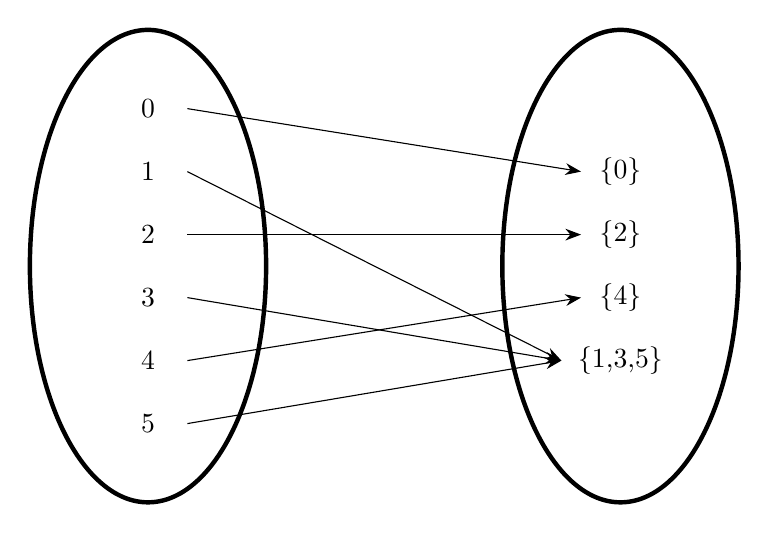
\begin{tikzpicture}
            \draw[ultra thick] (-3,0) ellipse (1.5 and 3);
            \node[] at (-3,2.0) {0};
            \node[] at (-3,1.2) {1};
            \node[] at (-3,0.4) {2};
            \node[] at (-3,-0.4) {3};
            \node[] at (-3,-1.2) {4};
            \node[] at (-3,-2.0) {5};

            \draw[ultra thick] (3,0) ellipse (1.5 and 3);
            \node[] at (3,1.2) {\{0\}};
            \node[] at (3,0.4) {\{2\}};
            \node[] at (3,-0.4) {\{4\}};
            \node[] at (3,-1.2) {\{1,3,5\}};

            \draw[-{Stealth[length=2mm]}] (-2.5,2.0) -- (2.5,1.2);
            \draw[-{Stealth[length=2mm]}] (-2.5,1.2) -- (2.25,-1.2);
            \draw[-{Stealth[length=2mm]}] (-2.5,0.4) -- (2.5,0.4);
            \draw[-{Stealth[length=2mm]}] (-2.5,-0.4) -- (2.25,-1.2);
            \draw[-{Stealth[length=2mm]}] (-2.5,-1.2) -- (2.5,-0.4);
            \draw[-{Stealth[length=2mm]}] (-2.5,-2.0) -- (2.25,-1.2);
        \end{tikzpicture}
    \end{center}
\end{itemize}

\section*{Problem 2}
\begin{itemize}
    \item [a.)] Given $X$ is equipped with the poset topology, the open subsets of $X$ are $\braces{5}$, $\braces{5,4}$, $\braces{5,4,3}$, $\braces{5,4,3,2}$, $\braces{5,4,3,2,1}$, $\braces{5,4,3,2,1,0}$, and $\varnothing$.

    \item [b.)] Given $X/{\sim}$ equipped with the quotient topology, the open subsets of $X/{\sim}$ are\break$\braces{\braces{0},\braces{2},\braces{4},\braces{1,3,5}}$, $\braces{\braces{2},\braces{4},\braces{1,3,5}}$, and $\varnothing$.

    \item [c.)] $p^{-1}(\braces{\braces{0},\braces{2},\braces{4},\braces{1,3,5}})=\braces{5,4,3,2,1,0}$\newline
    $p^{-1}(\braces{\braces{2},\braces{4},\braces{1,3,5}})=\braces{5,4,3,2,1}$\newline
    $p^{-1}(\varnothing)=\varnothing$

\end{itemize}

\section*{Problem 3}
Let $V\subset X/{\sim}$ be open, then by definiton $p^{-1}(V)$ is open, thus $p$ is continuous. $\blacksquare$

\end{document}
